% !TEX program = xelatex
\documentclass[12pt, a4paper]{article}
\usepackage[utf8]{inputenc}

\usepackage{fontspec}
\setmainfont[Ligatures=TeX]{Linux Libertine O}

\usepackage[hidelinks, colorlinks = true, linkcolor = black, urlcolor = blue]{hyperref}
\usepackage{indentfirst}
\usepackage{graphicx}
\usepackage[left=1cm,right=1cm,top=2cm,bottom=2cm]{geometry}
\usepackage{lipsum}
\usepackage{caption}
\usepackage{subcaption}
\usepackage{dirtytalk}

\title{\textbf{Ηλεκτρονική 3} \\ \textbf{Εργασία Τελεστικού Ενισχυτή}}
\author{Θεόδωρος Κατζάλης \\ ΑΕΜ:9282 \\ katzalis@auth.gr}
\date{12 Ιανουάριου 2020}


\begin{document}

\maketitle
\sloppy
\tableofcontents
\pagebreak

\section{Εισαγωγή}

Ο τελεστικός ενισχυτής που θα επιχειρήσουμε να σχεδίασουμε είναι 2 σταδιών με είσοδο ΝMOS χώρις στάδιο εξόδου και με χωρητικό φορτίο. Αξίζει βέβαια να σημειωθεί ότι συνήθως προτιμάται η χρήση PMOS εισόδου εξαιτίας επίδρασης υποστρώματος κλπ.

Ο τελεστικός είναι πάντα 2 βαθμίδων; Γιατί χρησιμοποιήσες nmos, πότε το ένα, πότε το άλλο.

Οι προδιαγραφές με βάση την εκφώνηση της άσκησης παραμετροποιημένες με το ΑΕΜ είναι οι ακόλουθες:
\subsection{Αρχικές Συνθήκες}

%\vspace{1cm}

\begin{table}[h!]
\centering
\begin{tabular}{|c|c|}
	\hline
	Προδιαγραφές & AEM=9282  \\
	\hline
	\textbf{CL} & 724 \\
	\hline
	\textbf{SR} & >709 \\
	\hline
	\textbf{Vdd} & 778 \\
	\hline
	\textbf{Vss} & -493 \\
	\hline
	\textbf{GB} & >493 \\
    \hline
    \textbf{A} & ?493 \\
    \hline
    \textbf{P} & 493 \\
    \hline
\end{tabular}
%\caption{}
\end{table}

\section{Περιγραφή αλγορίθμου (θεωρητική ανάλυση)}

Όσον αφορά το υπολογιστικό, θεωρητικό κομμάτι της σχεδίασης του τελεστικού ενισχυτή, ακολουθώντας τα βήματα απο τις σημειώσεις του μαθήματος, έχουμε να αναφερουμε τα εξής:

\subsection{Υπολογισμός σταθερών}

'Οσον αφορά την τάση κατωφλίου για τα MOS τραζίστορ, χρησιμοποιήσαμε τις τιμές που αναγράφονται στην περιγραφή των τρανζιστορ (KP), το οποίο θα μπορούσαμε να το υπολογίσουμε και χειροκίνητα με τον τύπο $C_{ox} = \mu_n \cdot \frac{\epsilon_{ox}}{t_{ox}}$, όπου  $\mu_n \equiv UO$ (spice model parameter). Πράγματι βλέπουμε ότι και με τους δύο τρόπους υπολογίζουμε τις ίδιες τιμές.
    
Επειδή δεν μας δίνεται κάποιο datasheet για τα συγκεκριμένα MOSFET προκειμένου να δούμε το έυρος του $V_{th}$ και τις μέγιστες και ελάχιστες τιμές, θεωρούμε ότι διατηρείται η τιμή σταθερή και ίση με αυτές που βρήκαμε απο την περιγραφή των μοντέλων. Δηλαδή $V_t(min) = V_t(max) = V_t$. Επίσης $V_{SB} = 0$ (zero body effect), οπότε $V_{to} = V_t$.

%Απο την άλλη ίσως θα μπορούσαμε να χρησιμοποιήσουμε το πινακάκι στις διαφάνεις +- 0.15

\subsection{Βήματα αλγορίθμου}    
\begin{enumerate}

    \item \textbf{Επιλογή τιμής L} (μήκος καναλιού). 
    
    Η τεχνολογία κατασκευής υποδηλώνει το ελάχιστο δυνατό μήκος καναλιού που μπορούμε να χρησιμοποποιήσουμε στην σχεδίαση μας και συνήθως επιλέγονται τιμές 1,5 ή 2 φορές αυτής της τιμής. Δεν μπορούμε βέβαια να χρησιμοποιήσουμε κάτι μικρότερο απο 0.35u. Για λόγους ευκολίας χρησιμοποιούμε την μονάδα.
    
    % Μatlab code here
    
    \item \textbf{Eπιλογή χωρητικότητας Miller}.
    
    Για να μην λειτουργεί ο ενισχυτής ως ταλαντωτής, σε συνδυασμό με την απόκλιση που μπορεί να έχει το κέρδος (βλέποντας την απόκριση συχνότητας), επίλεγεται phase margin 60 μοιρών, το οποίο απαιτεί να ικανοποιούνται οι εξής δύο συνθήκες: 
    \begin{itemize}
        \item $C_c > 0.22C_L$
        \item $g_{m6} > 10g_{m1}$
    \end{itemize}
    
    %Επιλέγουμε $C_c = 0.6204$ και δεν στρογγυλοποιούμε την τιμή, διότι αλλιώς δεν ικανοποιείται η δεύτερη συνθήκη, για την οποία θα γίνει λόγος στην συνέχεια.
    
    Επιλέγουμε $C_c = 0.6204\approx1$. 'Επειτα την στρογγυλοποίηση, όπως θα δούμε και στην συνέχεια, η δεύτερη συνθήκη δεν ισχύει για την δεδομένη τιμή $g_{m1}$, οπότε τελικά θα θεωρήσουμε $g_{m6} = 10g_{m1}$.
    
    \item Ρεύμα πόλωσης $Iref = I5 = I8$ ($I_7 \neq I_{ref}$, εξαιτίας συνθήκης για DC offset)
    
    \item Εύρεση $S_3 = (W/L)_3$. Βρίσκουμε $\leq1$, οπότε $S_3 = 1$.
    
    \item Έλεγχος $p_3 > 10 GB$.
    
    \item
\end{enumerate}

\subsection{Τελικές τιμές}

Πινακάκι για ρεύματα και W.

\section{Προσομοίωση SPICE}

Χρησιμοποιήσαμε για NMOS και PMOS τα μοντέλα mbreakN3 και mbreakP3 αντίστοιχα ($V_{SB} = 0$).

\begin{figure}[h!]
	\centering
	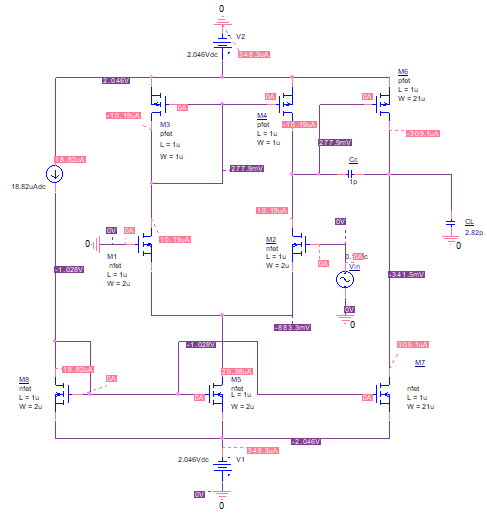
\includegraphics[width = \textwidth, height = .4\textheight, keepaspectratio]{assets/base.png}
	\caption{Κύκλωμα προσομοίωσης τελεστικού ενισχυτή}
\end{figure}

\subsection{Έλεγχος προδιαγραφών}

Για να βρούμε το κέρδος τάσης και το εύρος κέρδους, κάνουμε AC sweep βάζοντας τον marker στην έξοδο, αλλά εμείς θέλουμε λόγο εξόδου με εισόδου, οπότε ο marker όμως δεν δείχνει μόνο τάση εξόδου εκεί που τον έβαλες; Άρα ίσως και να μην θέλει marker και έπειτα να βάλεις trace Ι guess. Προσθέτουμε και την γωνία του κέρδους για να αποφανθούμε σχετικά με το περιθώριο φάσης.


\section{Tuning}


\end{document}
